\appendix
\section{Additional benchmark details}

\subsection{Functional hard-assignment control}
\label{app:functional}

This conditional MNIST control starts from the source-selected
indexator and its fitted source parameters. Let $J$ be its signed
representation, and let $V_\tau^{\mathrm{num}}$ be the source
numerical-selection sample. At fixed task parameters, write
\begin{equation}
    g_{\tau,p}:=\frac{\partial
        \mathcal L_{V_\tau^{\mathrm{num}}}}{\partial w_{\tau,p}},
    \qquad
    h_{\tau,p}:=\frac{2}{n_\tau O}
        \sum_{n,o}\left(
            \frac{\partial f_{\tau,o}(x_n)}{\partial w_{\tau,p}}
        \right)^2,
    \label{eq:benchmark-functional-ggn}
\end{equation}
where $n_\tau=|V_\tau^{\mathrm{num}}|$ and $O$ is the output dimension.
For a replacement $j\in\{0,\pm1,\ldots,\pm m\}$, define
$q_\tau(j):=\operatorname{sign}(j)c_{\tau,|j|}$, with $q_\tau(0)=0$,
and $\delta_{\tau,pj}:=q_\tau(j)-q_\tau(J_p)$. The shared proposal is
\begin{equation}
    j_p^+\in\operatorname*{arg\,min}_j
        \frac1T\sum_\tau
        \left(g_{\tau,p}\delta_{\tau,pj}
            +\frac12h_{\tau,p}\delta_{\tau,pj}^2\right).
    \label{eq:benchmark-functional-move}
\end{equation}
This diagonal Gauss--Newton score is a proposal surrogate, not an exact
loss change for a nonlinear network or simultaneous replacements.
The actual numerical-selection loss must decrease before a proposed
packet is accepted.
Write $R(J,\eta):=T^{-1}\sum_\tau
\mathcal L_{V_\tau^{\mathrm{num}}}(f_{J,\eta_\tau})$.

\begin{algorithm}[htbp]
    \small\DontPrintSemicolon\SetAlgoNoEnd
    \KwIn{Source-selected $J$, fitted numerical parameters
        $\{\eta_\tau\}$, source fitting and numerical-selection data.}
    $\mathcal B_{\mathrm f}\leftarrow\{J\}$\;
    \For{$k=1,\ldots,400$}{
        $\eta_\tau\leftarrow$ 20 Adam updates on
            $\mathcal L_{S_\tau^{\mathrm s}}$ at fixed $J$, for all $\tau$\;
        Compute $g_{\tau,p},h_{\tau,p}$ and $j_p^+$ by
            \eqref{eq:benchmark-functional-ggn}--\eqref{eq:benchmark-functional-move}\;
        Order profitable replacements by their predicted loss decrease\;
        $a\leftarrow0$\;
        \For{$b\in(64,32,16,8,4,2,1)$}{
            $J'\leftarrow J$ with its first $b$ profitable replacements\;
            \If{$R(J',\eta)<R(J,\eta)$}{
                $(J,a)\leftarrow(J',1)$; \textbf{break}\;
            }
        }
        \If{$a=0$}{
            $\mathcal N_{16}\leftarrow\{J\text{ with one of its first
                16 profitable replacements}\}$\;
            \tcp{Actual loss rescues a misleading quadratic ordering.}
            $J\in\operatorname*{arg\,min}_{J'\in\mathcal N_{16}\cup\{J\}}
                R(J',\eta)$\;
        }
        Retain distinct trajectory checkpoints in $\mathcal B_{\mathrm f}$\;
    }
    Refit the finite bank and select by
        \eqref{eq:method-structure-selection}\;
    \caption{Conditional functional proposal refinement}
\end{algorithm}

Four numerical learning rates, $0.0003,0.001,0.003,0.01$, are run;
seven distinct candidates including the unchanged baseline receive
common refitting. Because the starting indexator was selected using
source structure-selection data, its reuse here makes those source
losses exploratory; the disjoint development and final target cohorts
remain separate. A preliminary attempt with an incorrect basis-scale
conversion was excluded before candidate export. In the corrected
attempt, the initial source predictor and its loss agree in both
representations. No target responses or reference parameters enter
this procedure. Development results rejected it before test scoring.

\subsection{Numerical and competitor controls}

Synthetic target adaptation uses 18 fresh Adam starts: learning rates
$0.003,0.01,0.03$, three bias-activity quantiles $0.1,0.5,0.9$, and two
random starts per setting. Numerical-selection data choose checkpoints
over 2000 updates; four retained starts receive up to 48 Gauss--Newton
updates. Dense receives the same budget, with its Adam checkpoint
reported separately. On real data, development tasks select one global
learning rate, quantile and update count; a target task uses a single
fresh start and only its support responses. The selected update counts
are 25/50 for Dense/ours on Omniglot and 225/250 on MNIST.

A stronger Yeh source-only control on one separate DeepSets pilot uses
100 rather than 20 following inner steps and an explicit spectrally
damped inner Hessian solve rather than a 20-term Neumann action.
Its source structure-selection MSE improves from 0.04854 to 0.04325
for MAP and from 0.02905 to 0.02507 for the continuous basis; our
pilot value is 0.001762. This limited control does not establish
optimal tuning of Yeh, and these source losses are not target results.

The image implementation eliminates code variables from the weighted
calibration solve before solving for column scales. Comparison against
the unreduced system on learned source descriptors gives relative
code difference $3.50\times10^{-13}$. Thus this computational reduction
preserves that conditional calibration objective; it does not add
structural information.

\subsection{Binary Pattern and additional heatmaps}
\label{app:binary}

\begin{table}[htbp]\centering\small
\begin{tabular}{lrr}\toprule
Method & Clean-source I & Noisy-source I\\\midrule
Dense Adam & 91.17 & 91.17\\
Random I & 58.43 & 58.43\\
LUT-Q I & 100.00 & 100.00\\
Yeh MAP I & 100.00 & 96.59\\
Yeh soft & 100.00 & 100.00\\
MSR-FC U & 99.31 & 95.83\\
Ours & 100.00 & 100.00\\
\bottomrule\end{tabular}
\caption{Binary Pattern follow-up: mean query accuracy (\%) over three families, with 512 support, 128 numerical-selection and 1408 held-out binary inputs. All numerical parameters are trained afresh by binary cross entropy. These structures were extracted from real-valued source functions, so this is not extraction from binary supervision alone.}
\label{tab:benchmark-binary}\end{table}


\begin{figure}[htbp]
    \centering
    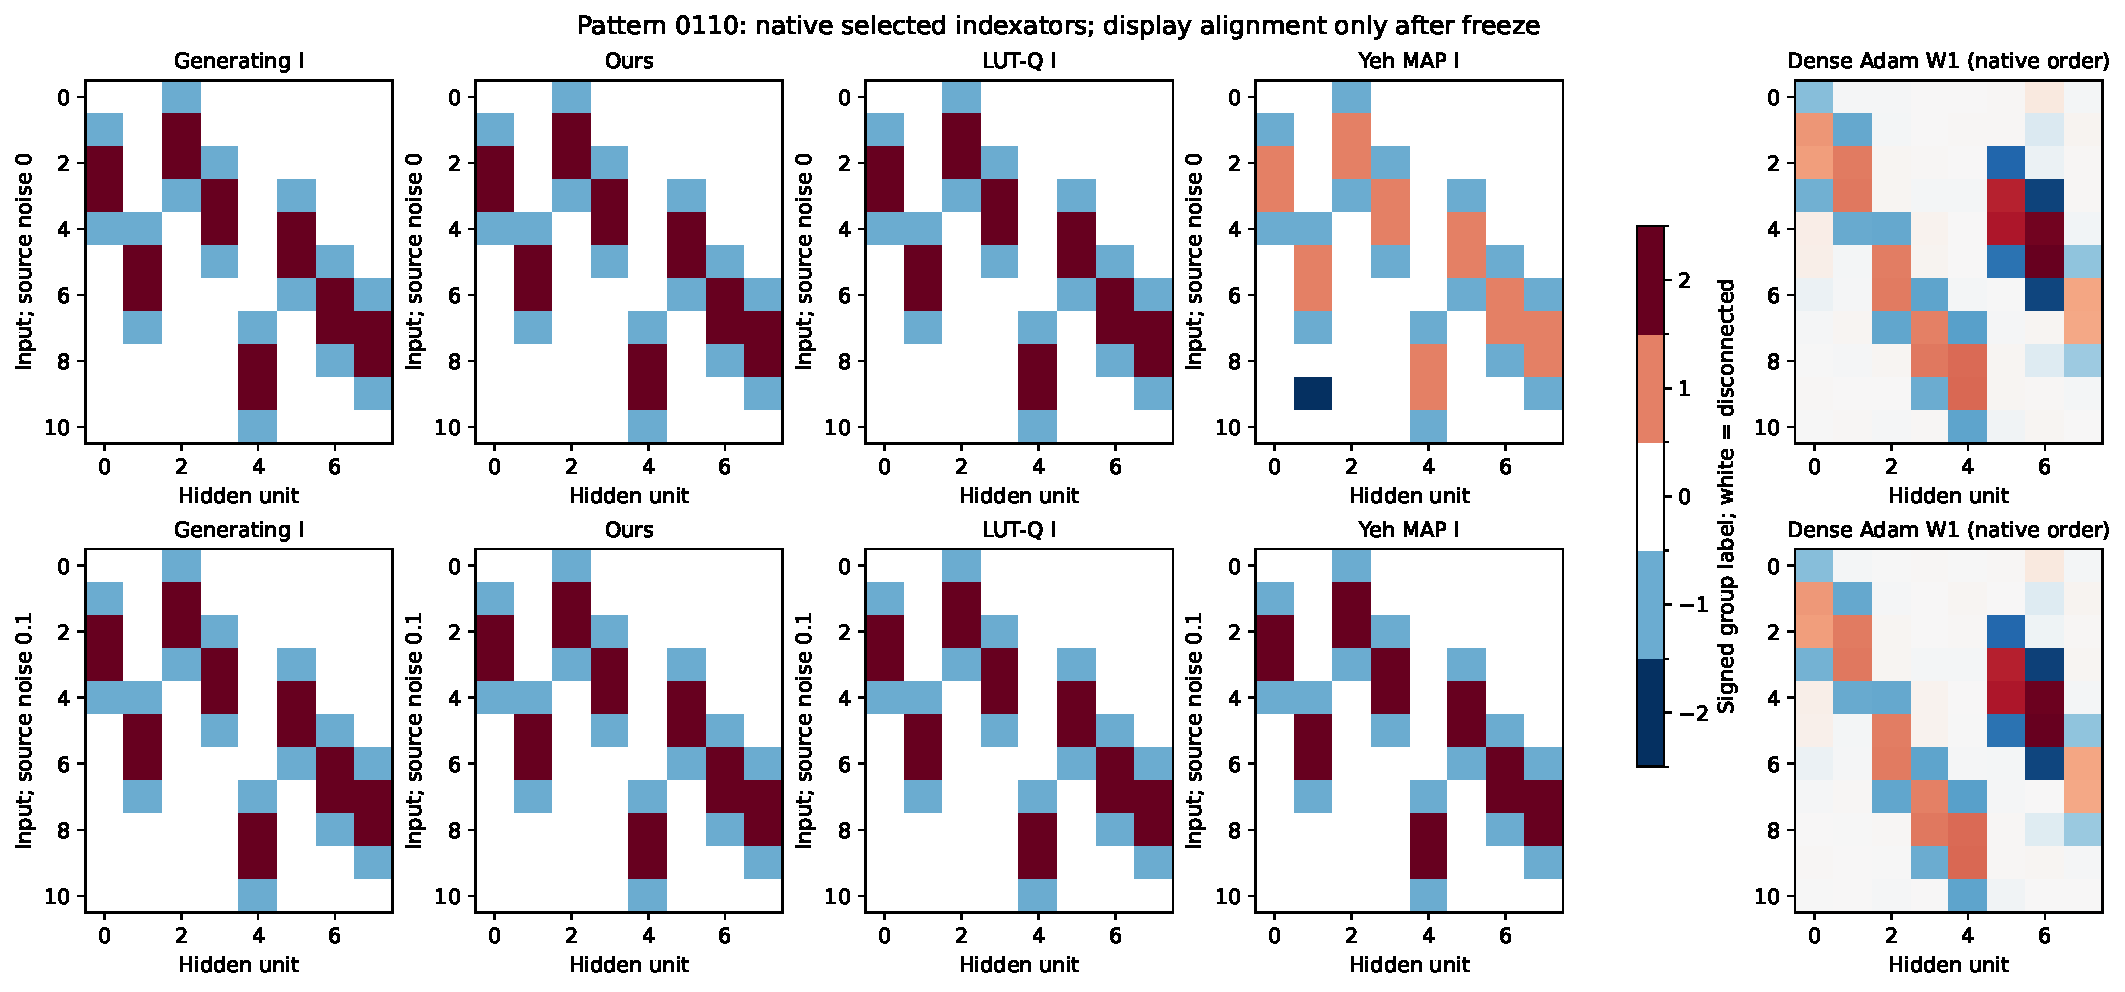
\includegraphics[width=\linewidth]{benchmark_pattern_heatmaps.pdf}
    \caption{Pattern indexators for the first registered family.
        Display alignment uses reference labels only after all
        predictions are frozen. Dense weights retain native unit order.}
\end{figure}

\begin{figure}[htbp]
    \centering
    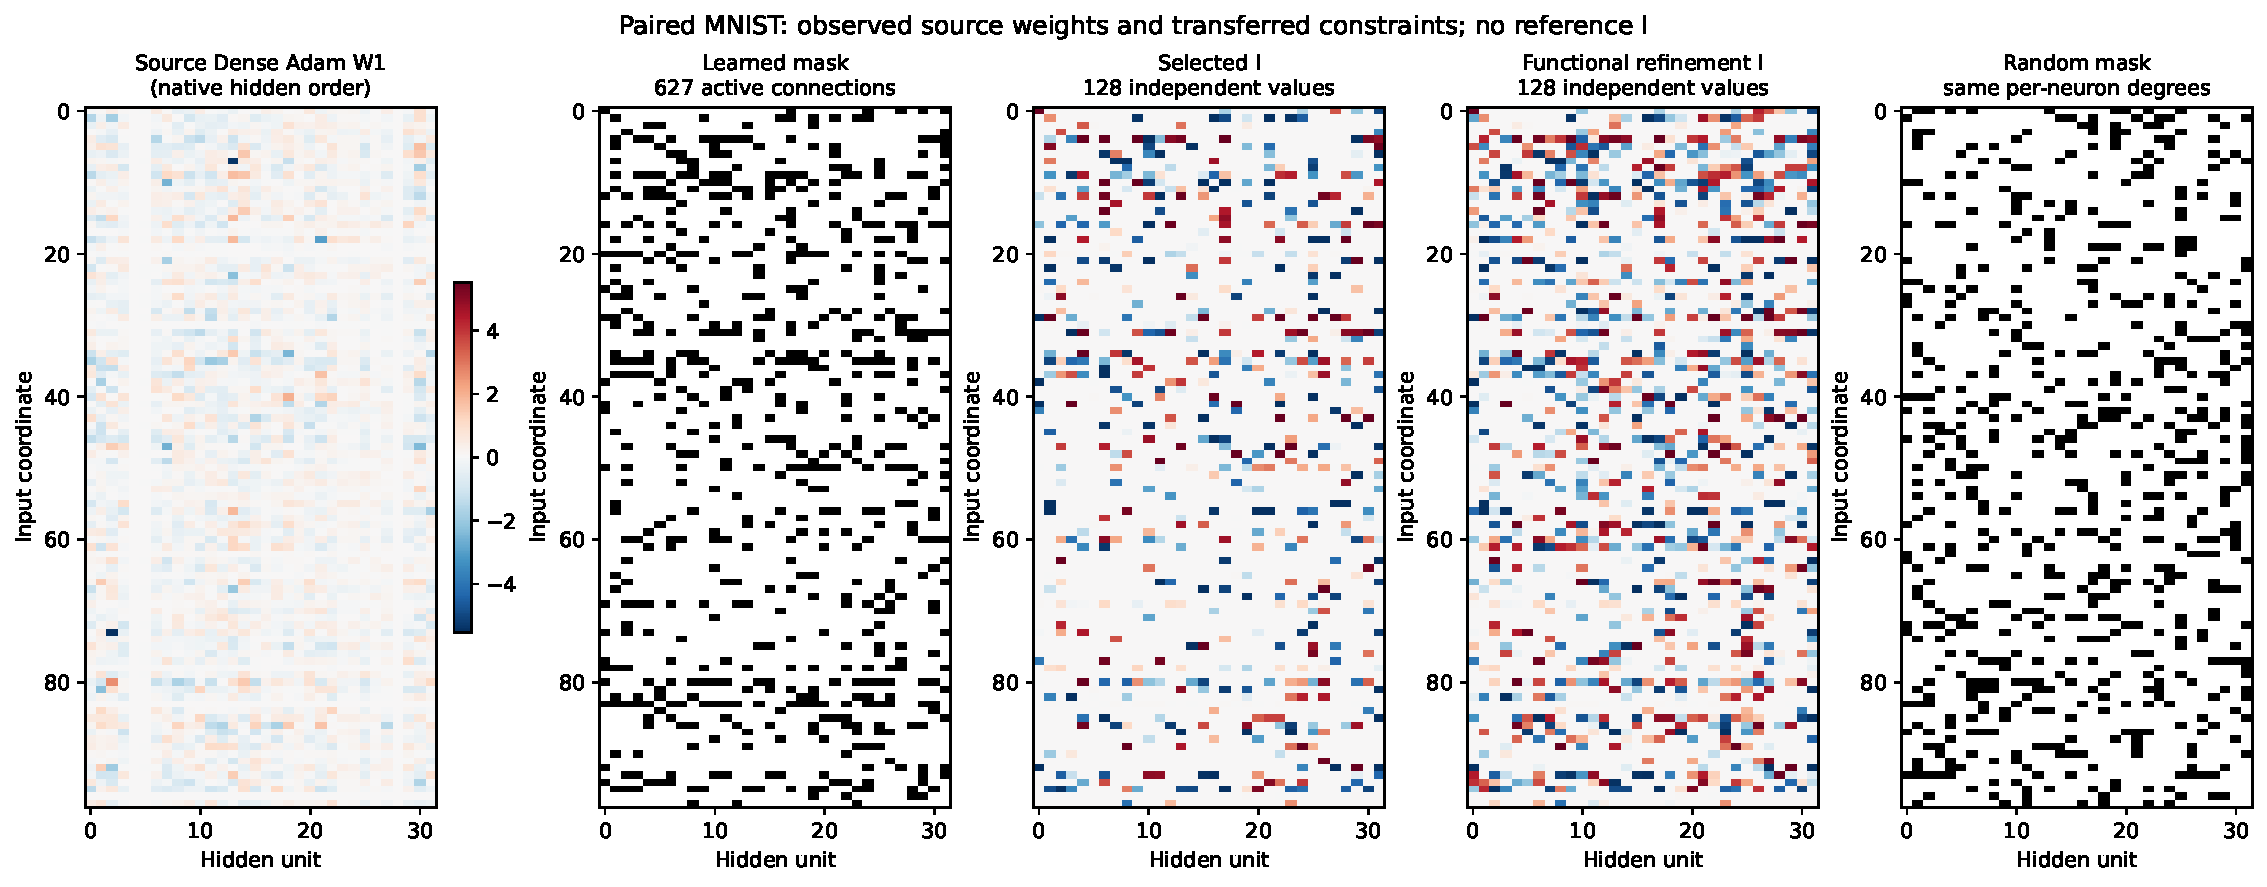
\includegraphics[width=\linewidth]{benchmark_mnist_heatmaps.pdf}
    \caption{Paired MNIST source weights, learned mask, selected signed
        indexator, functional control and degree-matched random mask.
        Group labels are names, not numerical weight magnitudes.
        Releasing weights in the learned mask changes the numerical
        budget from 128 to 627; no reference indexator is available.}
\end{figure}

\subsection{Measured computational costs}
\label{app:costs}

Offline costs include required dense preparation, all configurations,
common source refitting and development selection. Continuous
competitors pay only for the dense preparation they use, rather than
the extra descriptor refinement required by discrete refitting.
The conditional functional row additionally includes the original
search and its diagnostic/refinement stages. Shared stages are counted
in each independent pipeline; summing rows would count them repeatedly.
Search seconds are measured with operator profiling under shared
scheduling and are not an isolated latency benchmark. The CPU parts
of calibration are timed but absent from the registered Torch counts.

Target timings are separate unprofiled runs, one process per GPU.
Synthetic rows measure the first registered family at 1024 fitting
examples; real rows measure the complete target cohort. Allocated
memory depends on packing: eight tasks for synthetic data and chunks
of up to 64 for images. Synthetic target operator counts in the CSV
cover all three support sizes, whereas its timing column covers only
1024; these scopes must not be combined as a single FLOP rate.
An unavailable Adam-only peak is left blank rather than replaced by
the later Gauss--Newton peak.
The target GFLOPs column reports work per task, including all numerical
starts and updates in the stated scope. FLOP/s is a throughput measure
and is not measured here. Unsupported Torch operations and CPU numerical
linear algebra are excluded from these counts.

\begin{table}[htbp]
\centering\small\setlength{\tabcolsep}{3.5pt}
\begin{tabular}{lrrrrrr}
\toprule
Method & Search s$^*$ & Search TFLOPs$^*$ & Target GFLOPs$^\dagger$ & ms/task & Target MiB & Search MiB\\
\midrule
Dense Adam & 0 & 0 & -- & 788 & -- & 0\\
Dense Adam + GN & 0 & 0 & 28.2 & 996 & 650 & 0\\
Random I & -- & -- & 4.5 & 969 & 44.5 & --\\
LUT-Q I & 198 & 2.86 & 4.52 & 948 & 44.5 & 926\\
Yeh MAP I & 443 & 3.43 & 4.52 & 955 & 44.5 & 926\\
Yeh soft & 364 & 1.43 & 4.49 & 955 & 44.5 & 833\\
MSR-FC U & 183 & 0.956 & 4.51 & 901 & 44.5 & 833\\
Ours & 119 & 1.97 & 4.52 & 963 & 44.5 & 926\\
\bottomrule\end{tabular}
\caption{Pattern 0110: measured computation. Target timing excludes the FLOP profiler and uses one process per GPU. $^*$Search seconds include profiling overhead and shared scheduling. $^\dagger$Target GFLOPs are per task: the complete 64/256/1024 sweep on synthetic data, one prescribed support budget on real data; synthetic time covers only 1024. These are incomplete Torch operation counts, not FLOP/s. A dash indicates unavailable measurement.}
\end{table}
\begin{table}[htbp]
\centering\small\setlength{\tabcolsep}{3.5pt}
\begin{tabular}{lrrrrrr}
\toprule
Method & Search s$^*$ & Search TFLOPs$^*$ & Target GFLOPs$^\dagger$ & ms/task & Target MiB & Search MiB\\
\midrule
Dense Adam & 0 & 0 & -- & 775 & -- & 0\\
Dense Adam + GN & 0 & 0 & 189 & 1212 & 3668 & 0\\
Random I & -- & -- & 19.8 & 948 & 136 & --\\
LUT-Q I & 293 & 20.5 & 20.1 & 943 & 136 & 3877\\
Yeh MAP I & 556 & 21.9 & 19.8 & 959 & 136 & 3877\\
Yeh soft & 400 & 6.09 & 19.9 & 966 & 136 & 3611\\
MSR-FC U & 191 & 4.5 & 19.9 & 962 & 136 & 3611\\
Ours & 533 & 20.4 & 20.2 & 993 & 136 & 3877\\
\bottomrule\end{tabular}
\caption{Synthetic DeepSets: measured computation. Target timing excludes the FLOP profiler and uses one process per GPU. $^*$Search seconds include profiling overhead and shared scheduling. $^\dagger$Target GFLOPs are per task: the complete 64/256/1024 sweep on synthetic data, one prescribed support budget on real data; synthetic time covers only 1024. These are incomplete Torch operation counts, not FLOP/s. A dash indicates unavailable measurement.}
\end{table}
\begin{table}[htbp]
\centering\small\setlength{\tabcolsep}{3.5pt}
\begin{tabular}{lrrrrrr}
\toprule
Method & Search s$^*$ & Search TFLOPs$^*$ & Target GFLOPs$^\dagger$ & ms/task & Target MiB & Search MiB\\
\midrule
Dense Adam & 31.9 & 6.31 & 0.0354 & 1.58 & 70.5 & 1067\\
Random I & -- & -- & 0.164 & 1.66 & 59.1 & --\\
LUT-Q I & 1704 & 20.9 & 0.0214 & 2.56 & 56.8 & 2426\\
Yeh MAP I & 3025 & 103 & 0.167 & 2.78 & 59.1 & 1176\\
Yeh soft & 3084 & 104 & 0.164 & 1.52 & 59.1 & 1176\\
MSR-FC U & 2080 & 55.6 & 0.167 & 2.59 & 59.1 & 705\\
Ours & 1313 & 15.9 & 0.167 & 2.75 & 59.1 & 705\\
MSR + learned init & 554 & 40.4 & 7.10e-03 & 0.476 & 57.5 & 705\\
\bottomrule\end{tabular}
\caption{Aug-Omniglot: measured computation. Target timing excludes the FLOP profiler and uses one process per GPU. $^*$Search seconds include profiling overhead and shared scheduling. $^\dagger$Target GFLOPs are per task: the complete 64/256/1024 sweep on synthetic data, one prescribed support budget on real data; synthetic time covers only 1024. These are incomplete Torch operation counts, not FLOP/s. A dash indicates unavailable measurement.}
\end{table}
\begin{table}[htbp]
\centering\small\setlength{\tabcolsep}{3.5pt}
\begin{tabular}{lrrrrrr}
\toprule
Method & Search s$^*$ & Search TFLOPs$^*$ & Target GFLOPs$^\dagger$ & ms/task & Target MiB & Search MiB\\
\midrule
Dense Adam & 27.8 & 7.74 & 1.52 & 30.9 & 71.3 & 213\\
Random I & -- & -- & 6.84 & 55.8 & 1096 & --\\
LUT-Q I & 1408 & 125 & 3.81 & 26.5 & 1096 & 1911\\
Yeh MAP I & 3057 & 263 & 5.33 & 40.9 & 1096 & 1911\\
Yeh soft & 3054 & 263 & 4.03 & 28.3 & 1096 & 1911\\
MSR-FC U & 2068 & 197 & 6.41 & 50.8 & 1096 & 1911\\
Ours & 1188 & 112 & 4.24 & 29.7 & 1096 & 1911\\
Ours + functional & 1605 & 175 & 5.98 & 46.3 & 1096 & 1911\\
Our mask, free weights & 1216 & 119 & 3.01 & 46.2 & 71.7 & 1911\\
Random mask, free weights & -- & -- & 2.85 & 44.8 & 71.7 & --\\
MSR + learned init & 534 & 45 & 0.0339 & 5.48 & 63.7 & 439\\
\bottomrule\end{tabular}
\caption{Paired MNIST sums: measured computation. Target timing excludes the FLOP profiler and uses one process per GPU. $^*$Search seconds include profiling overhead and shared scheduling. $^\dagger$Target GFLOPs are per task: the complete 64/256/1024 sweep on synthetic data, one prescribed support budget on real data; synthetic time covers only 1024. These are incomplete Torch operation counts, not FLOP/s. A dash indicates unavailable measurement.}
\end{table}


\begin{figure}[htbp]
    \centering
    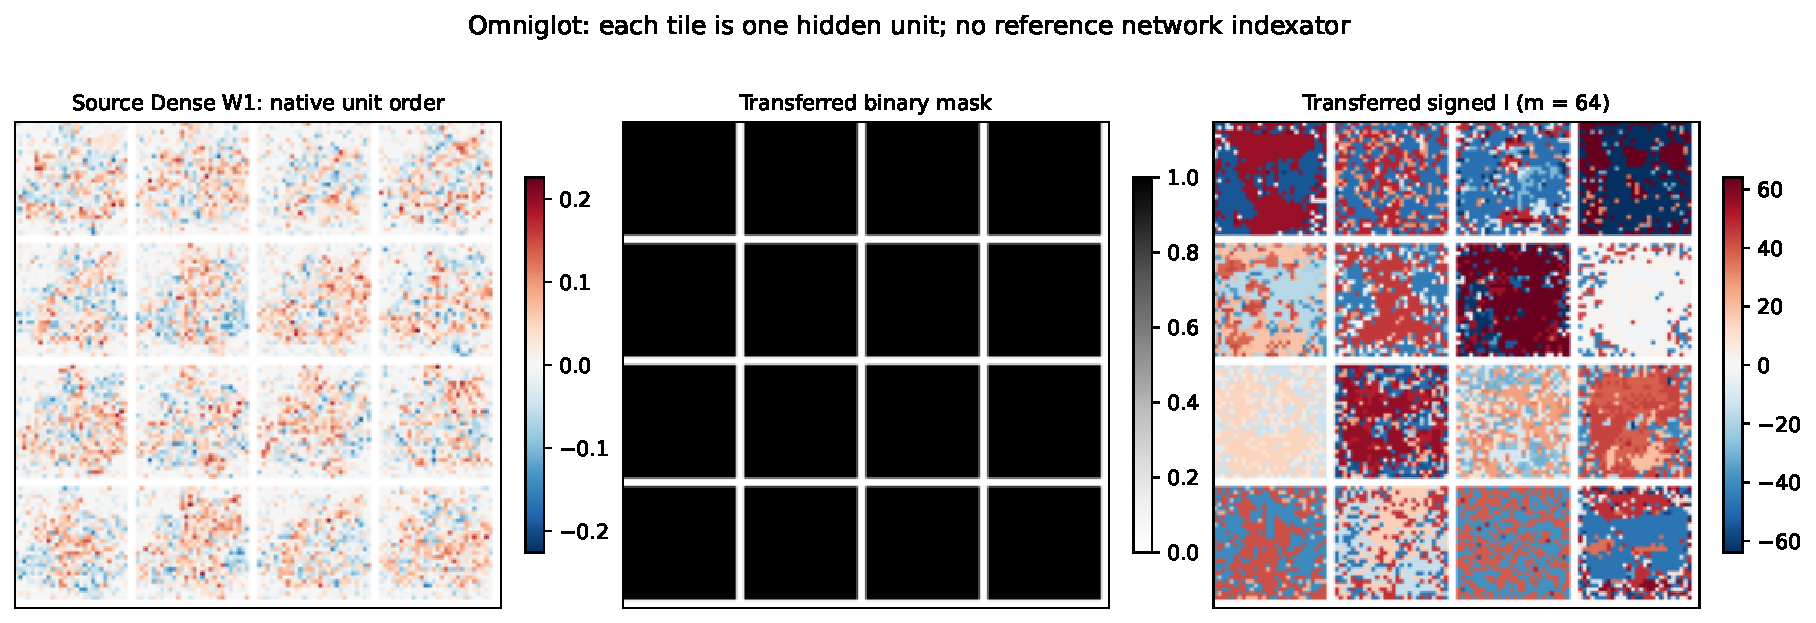
\includegraphics[width=\linewidth]{benchmark_omniglot_heatmaps.pdf}
    \caption{Omniglot source weights, transferred mask and signed
        indexator, with one $28\times28$ tile per hidden unit.
        Hidden-unit orders are native to each model; numerical weights
        and arbitrary group labels have separate color scales.}
\end{figure}
